
%%%%%%%%%%%%%%%%%%%%%%%%%%%%%%  IEEEsample2e.tex %%%%%%%%%%%%%%%%%%%%%%%%%%%%%%
%% changes for IEEEtrans.cls marked with !PN
%% except all occ. of IEEEtran.sty changed IEEEtran.cls
%%%%%%%%%%                                                       %%%%%%%%%%%%%
%%%%%%%%%%    More information: see the header of IEEEtran.cls   %%%%%%%%%%%%%
%%%%%%%%%%                                                       %%%%%%%%%%%%%
%%%%%%%%%%%%%%%%%%%%%%%%%%%%%%%%%%%%%%%%%%%%%%%%%%%%%%%%%%%%%%%%%%%%%%%%%%%%%%%

\documentclass[journal,transmag]{IEEEtran}
%\documentclass[twocolumn]{IEEEtran} %!PN
%\documentclass[12pt,draft]{IEEEtran} %!PN
%\documentstyle[twocolumn]{IEEEtran}
%\documentstyle[12pt,twoside,draft]{IEEEtran}
%\documentstyle[9pt,twocolumn,technote,twoside]{IEEEtran}
\usepackage{graphicx}
%\graphicspath{{../figures/}{fig_site/}}

\def\BibTeX{{\rm B\kern-.05em{\sc i\kern-.025em b}\kern-.08em
    T\kern-.1667em\lower.7ex\hbox{E}\kern-.125emX}}

\newtheorem{theorem}{Theorem}
\setcounter{page}{100}

\begin{document}

%\title{Using the Style File IEEEtran.sty} 
\title{Using the Document Class IEEEtran.cls in the EELT-7019} %!PN

\author{Gerry Murray, Silvano Balemi\thanks{S. Balemi is with the
Automatic Control Laboratory, Swiss Federal Institute of Technology
(ETH), Zurich, Switzerland. E-mail: balemi@aut.ee.ethz.ch .}\thanks{Note
that the ``thanks'' command does no longer produce footnote marks.}}

%\markboth{IEEE Transactions On Automatic Control, Vol. XX, No. Y, Month 2020}
\markboth{IEEE Transactions On Artificial Intelligence, Vol. XX, No. Y, December 2020}
%{Murray and Balemi: Using the style file IEEEtran.sty} %!PN
{Murray and Balemi: Using the Document Class IEEEtran.cls} %!PN


\maketitle
%\thispagestyle{plain}\pagestyle{plain}

\begin{abstract}
This article explains how to use a \LaTeX\ style that produces a good
approximation to the style used in the IEEE Transactions.  The article
is itself an example of the IEEEtran.cls style in action.
\end{abstract}

\begin{IEEEkeywords}
    IEEEtran, journal, \LaTeX, magnetics, paper, template.
\end{IEEEkeywords}

\section{Introduction}
\IEEEPARstart{T}{he} Institute of Electrical and Electronics Engineers
Inc. (IEEE in short) publishes a large number of journals.  Some of
these these are

%% NOTE: "\itemindent -1em \leftmargini 2em" . Sometimes other values
%% are used, e.g. "\itemindent 2em \leftmargini 0em"
\begin{itemize}
\item IEEE Transactions on Automatic Control
\item IEEE Transactions on Software Engineering
\item IEEE Transactions on Communications
\item IEEE Transactions on Industrial Electronics
\item IEEE Transactions on Systems Man and Cybernetics
\item IEEE Transactions on Circuits and Systems
\item IEEE Transactions on Robotics and Automation
\item IEEE Transactions on Computers
\item \ldots{}
\end{itemize}

Authors who have prepared their articles using \LaTeX\
can get them formatted in a style identical to that of a typical paper
in one of those journals.

The aim of the style file {\tt IEEEtran.cls} is to allow authors of
papers to estimate the page count and facilitate input-processing of
the compuscript.  The style file {\tt IEEEtran.cls} can be used
together with the bibliography style file {\tt IEEE.bst}.

IEEE has sophisticated software, in house and different to \LaTeX,
which they use to typeset transaction papers. The single most
important reason for this style file was due to the fact that many
authors (using \TeX\ and \LaTeX) were supplying their compuscripts
using style files that were {\em single column page wide}. It was
obvious from the coding that many had spent time inserting commands
that made the displayed equations ``pretty'', spreading them right
across the page.  But of course, IEEE transactions are {\em double
column}, with the column width being 21 pica. Thus, the IEEE publishing
staff ended up deleting these typesetting `niceties' and breaking the
page wide displayed equations so that they would {\em fit} inside the
style-required 21 pica. By using this style file you'll find that the
displayed equations, algorithms, nomenclature lists, etc. that you
supply to us (on disk or via e-mail: ask the editor of your
transactions) will undergo minimal change.
%


\section{How to Use the File IEEEtran.cls}
This style file has been written so to allow, with very few changes,
the formatting of input that is suitable for the \LaTeX\ {\tt article}
style.
First,  the \verb+IEEEtran.cls+ style file has to be
selected with a command of the form
\begin{center}
%\verb+\documentstyle[twocolumn,twoside]{IEEEtran}+ %!PN
\verb+\documentclass[twocolumn,twoside]{IEEEtran}+
\end{center}

The default font size is 10 points.  The default page style has been
redefined and is now set by {\tt IEEEtran.cls} to ``\verb+headings+''.

IEEE Transactions papers do not include author affiliations below or beside
the name(s) of the author(s); instead, use the command
\verb+\thanks{...}+ to list addresses. Note that the
\verb+\thanks{..}+ command in the title no longer produce marks:
the thanks-footnote should therefore be self-contained, with address
and name of the author(s).

Footnotes produce a footnote mark as usual.\footnote{The footnote is
indicated by a footnote mark}

The command ``\verb+\PARstart{X}{YYY} ZZZ+'' produces a large letter
\verb+X+ at the beginning of the paragraph. The string \verb+YYY+
will be automatically changed to capital letters.

The bibliography style file {\tt IEEE.bst} allows \BibTeX\ to include
the references from the chosen bibliography file(s) according to the
format required by IEEE Transactions.

Full papers should include the biography of the authour.
An example of a formatted biography is given at the end of
this sample article.
The environment is called \verb+biography+ and requires the
name of the person whose bio\-graphy is presented.

In Fig. \ref{fg:gradiente_matlab} we can see an example for the definition of
the title page and of the main commands needed to compile a \LaTeX
file with IEEEtran.cls.

The command \verb+\markboth{leftTEXT}{rightTEXT}+ can be used for
setting the running heads. If the option {\tt twoside} is not
selected, both even and odd headers will display {\tt leftTEXT}
together with the page number.  Note that the header of the title page
always displays {\tt leftTEXT} as it bears the journal name.

\subsection{Additional Changes}
Most changes resulting from the use of IEEEtran.cls should be
transparent to the user. For instance,
captions for figures and tables have been modified. Caption of
tables, however, should be defined before the table item.

\begin{figure}[hbt]
\begin{center}
\setlength{\unitlength}{0.0105in}%
\begin{picture}(242,156)(73,660)
\put( 75,660){\framebox(240,150){}}
\put(105,741){\vector( 0, 1){ 66}}
\put(105,675){\vector( 0, 1){ 57}}
\put( 96,759){\vector( 1, 0){204}}
\put(105,789){\line( 1, 0){ 90}}
\put(195,789){\line( 2,-1){ 90}}
\put(105,711){\line( 1, 0){ 60}}
\put(165,711){\line( 5,-3){ 60}}
\put(225,675){\line( 1, 0){ 72}}
\put( 96,714){\vector( 1, 0){204}}
\end{picture}
\end{center}
\caption{This is a sample figure. The caption comes after the figure.}
\end{figure}

A Fig. \ref{fg:gradiente_matlab} foi utilizada na aula de redes neurais.

\begin{figure}[htb!]%--------------------------------------------
\begin{center}
    %\fbox{
    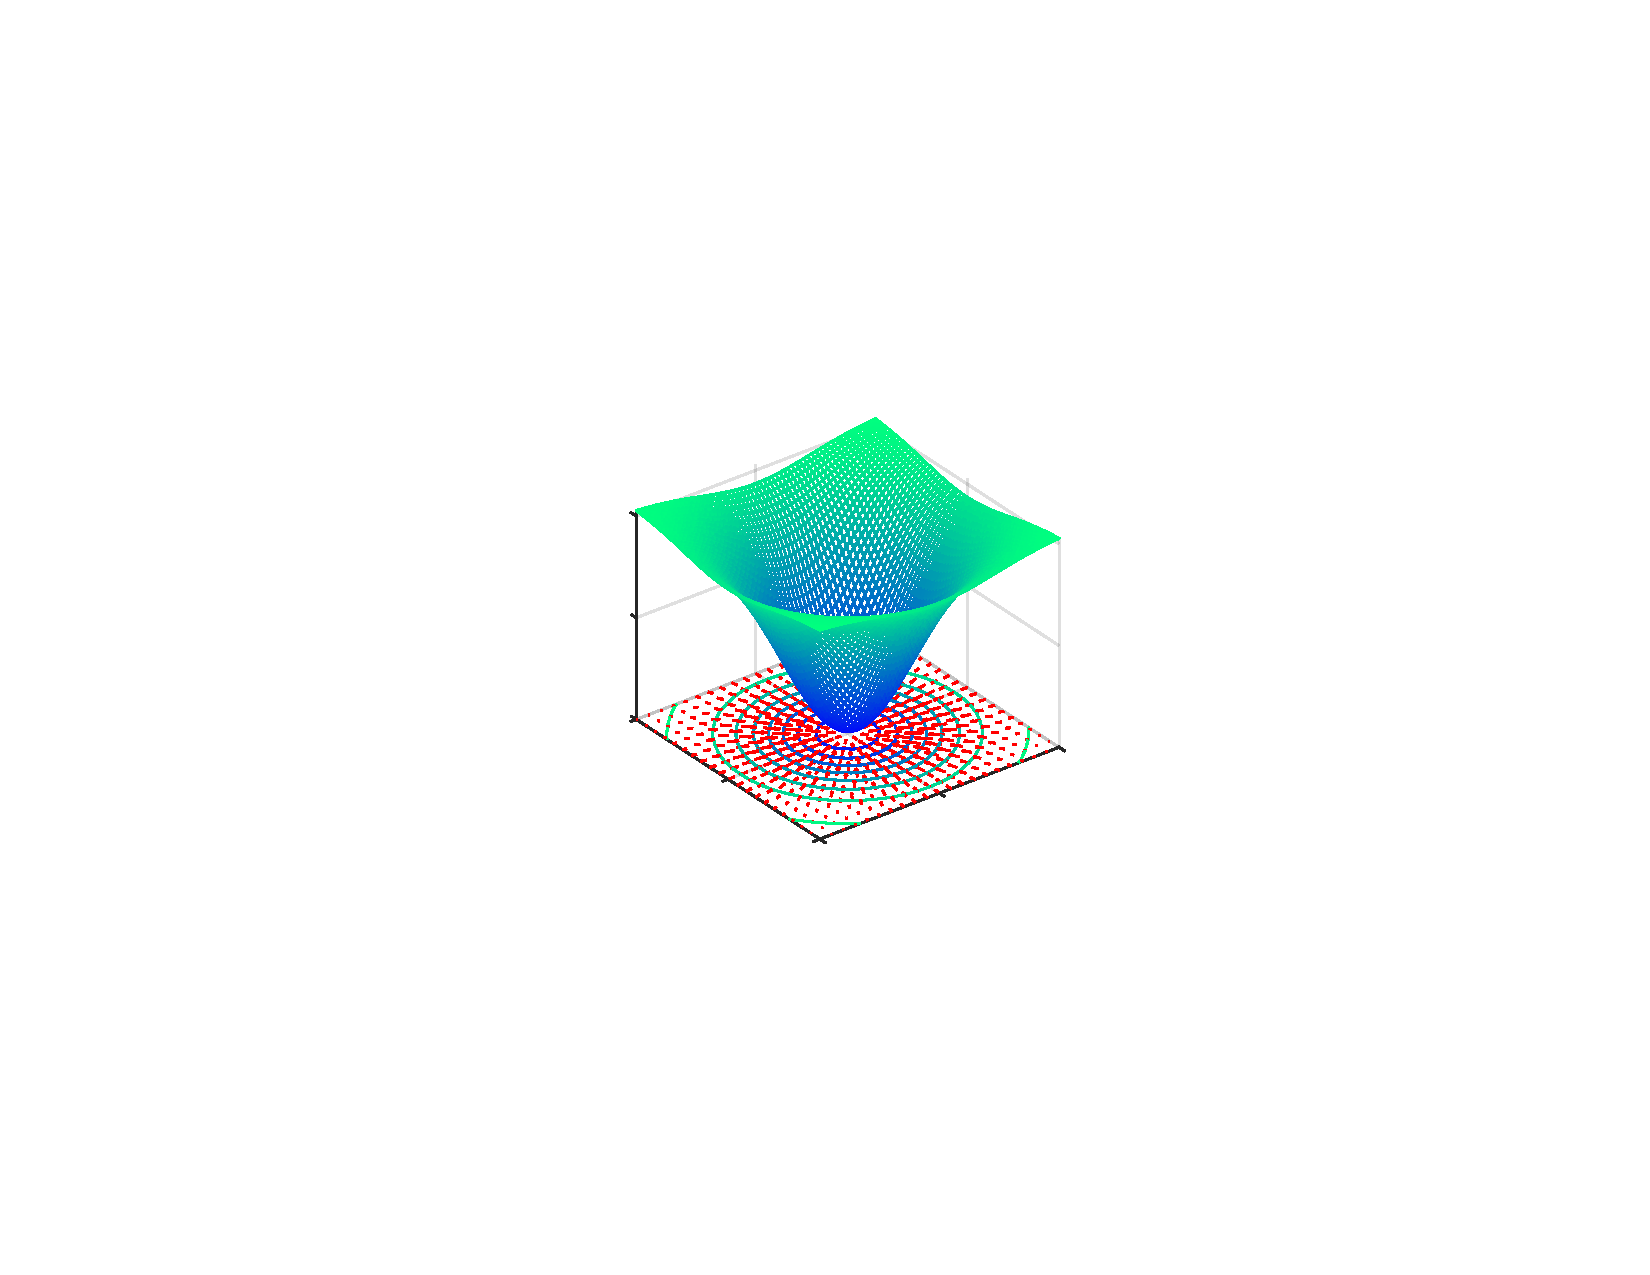
\includegraphics[scale = 0.9, trim = 107.0mm 73.0mm 100.0mm 70.0mm,clip]{Gradiente_Matlab.pdf}
    % }
    \caption{This is a sample figure utilizada na aula de redes neurais. The caption comes after the figure.}
    \label{fg:gradiente_matlab} % nome da figura
\end{center}
\end{figure}

\begin{table}[htb]
\caption{The Caption Comes Before the Table.}
\begin{center}
{\tt
\begin{tabular}{|c||c|c|c|}\hline
&title page&odd page&even page\\\hline\hline
onesided&leftTEXT&leftTEXT&leftTEXT\\\hline
twosided&leftTEXT&rightTEXT&leftTEXT\\\hline
\end{tabular}
}
\end{center}
\end{table}

\subsubsection{Environments}
The environments for theorem, propositions, lemmas, etc. can be
defined with the usual \LaTeX\ \cite{LaTeX,LaTeXD} command
\verb+\newtheorem{..}{..}+.  The proof environment is already defined.

\begin{theorem}[Theorem name]
Consider the system
\begin{equation}
\begin{array}{rrr}
\dot x&=&A.x+B.u\\[2mm]
y&=& C.x+D.u
\end{array}
\end{equation}
If $A$ is stable, then the pair $\{A,B\}$ is stabilizable. Moreover,
this holds for any $B$.
\end{theorem}
\begin{IEEEproof}
    The proof is trivial.
\end{IEEEproof}

\subsection{Preparing a Technical Note}
A technical note can be prepared using the additional option
\verb+technote+ in the documentstyle command. Note that the default
point size is still 10 points, but that 9 points should be selected.
The format for a technical note can thus be selected with a command
of the form
\begin{center}
%\verb+\documentstyle[...side,9pt,technote]{IEEEtran}+
\verb+\documentclass[...side,9pt,technote]{IEEEtran}+ %!PN
\end{center}
All the definitions and commands are still valid  even after the
changes caused by the option \verb+technote+.

\subsection{Submitting a Paper}
The paper can be prepared for submission by omitting the option {\tt
twocolumn} and choosing the option {\tt draft} (this will modify the
baselinestretch variable).
Thus, the format for submission contains a definition of the form
\begin{center}
%\verb+\documentstyle[...side,12pt,draft]{IEEEtran}+
\verb+\documentclass[...side,12pt,draft]{IEEEtran}+ %!PN
\end{center}

\section{Optional Formatting}

When you are happy with the {\em ultimate unequivocal final version},
you may perform following additional changes.

\subsection{``Hard-Coding'' Symbolics}
Change the symbolics so that the file actually contains the reference
numbers
{\em i.e.\ \/}``\verb+... \cite{fred:88} ...+'' should be changed to
``\verb+... [3] ...+''. One author (who used the style file) did a smart
thing
{\em after\/} he had decided upon a final version.  He put his
\verb+\cite{..}+ command and other symbolics on a line on their own
and commented them out (from the formatting) by putting a \verb+%+
sign before each symbolic. Then, on the next line he just inserted the
copy-matching numerical, like this:

\begin{verbatim}
    Well, according the Fred Bloggs
    %\cite{fred:88}
    [24]
    the value of $\alpha$ should be even
    greater than what we think it should be.
\end{verbatim}

Thus, {\em he\/} knows he put in the correct (copy-matching) numerical and
the IEEE publishing staff can send him back an author-proof
that correctly matches his submission.

The above also applies to the referencing of table and figures
(and any ``auto-numbering'' feature, standard or synonymous with your
system).

Figure captions can be part of the text (in between paragraphs) like this:

\begin{verbatim}
    And in Fig. 3 we see that the
    value of $\alpha$ increases exponentially.

       Fig. 3\quad This is the caption for
       figure 3 showing some $\alpha$.

    And after the caption we continue on
    with the next paragraph, like this.
\end{verbatim}

In essence, by you actually putting in the {\em correct copy
matching\/} numericals so that no problems arise with incomplete files
being sent to the transactions (the wrong \verb+*.bib+, \verb+*.bbl+ files,
the wrong versions of figures etc).  Also, and more importantly, the
numbers that are on your hard-copy (and in the reviewer's hands) will
be the same ones that you receive in your author proof.

\subsection{Including the Bibliography into the \LaTeX\ Source File}
You can reduce the number of files you have to send to the IEEE
publishers in the following way. Run \BibTeX\ on the
\verb+*.aux+ file. This creates a \verb+*.bbl+ file: include this
into your \LaTeX\ source file at the place where you defined the
\verb+\bibliography{..}+ command  and comment this command out.
Remove the \verb+*.bbl+ file.  Then, your \LaTeX\ file will include
all the necessary information about your bibliography and no \verb+*.bbl+
or \verb+*.bib+ file will be needed.

This may seem like an awful lot of work... but not really..
This will allow to process your paper quickly and efficiently, and assure
you
that what you send in {\em will\/} actually be sent back to you
without  mistakes (cites, refs etc.).

\section{Conclusions}
This sample article has presented the style file IEEEtran.cls
This file can be especially useful in preparing articles for
submission and for preparing the final version to be sent to the IEEE
publishers.

In essence, the style file ``IEEEtran.cls'' is not really for
formatting (paper printout) -- but is for IEEE {\em
input processing\/} which is chalk and cheese, frankly.


\section*{Acknowledgments}
The authors would like to acknowledge the suggestions of many people.


\nocite{*}
\bibliographystyle{IEEE}
%%%%%\bibliography{bib-file}  % commented if *.bbl file included, as
%%%%%see below


%%%%%%%%%%%%%%%%% BIBLIOGRAPHY IN THE LaTeX file !!!!! %%%%%%%%%%%%%%%%%%%%%%%%
%% This is nothing else than the IEEEsample.bbl file that you would         
%%
%% obtain with BibTeX: you do not need to send around the *.bbl file        
%%
%%---------------------------------------------------------------------------%%
%
\begin{thebibliography}{1}
\bibitem{LaTeX}
Leslie Lamport,
\newblock {\em A Document Preparation System: \LaTeX, User's Guide and
  Reference Manual},
\newblock Addison Wesley Publishing Company, 1986.
\bibitem{LaTeXD}
Helmut Kopka,
\newblock {\em \LaTeX, eine Einf\"uhrung},
\newblock Addison-Wesley, 1989.
\bibitem{TeX}
D.K. Knuth,
\newblock {\em The {\rm T\kern-.1667em\lower.7ex\hbox{E}\kern-.125emX}book},
\newblock Addison-Wesley, 1989.
\bibitem{METAFONT}
D.E. Knuth,
\newblock {\em The {\rm METAFONT}book},
\newblock Addison Wesley Publishing Company, 1986.
\end{thebibliography}
%
%%---------------------------------------------------------------------------%%

\begin{IEEEbiography}{Gerry Murray} will process your compu\-script,
adding ``value'' to your \LaTeX\ file using a sophisticated text
editor. Jeremy Barth will standardize the dimensions you've used, run
a spell check, apply SGML tags to structure your document and validate
all coding. The editor will ``on-screen edit'' the file, ``size'' your
artwork and supply you with a laser proof by mail, or by fax, or even
e-mail you a postscript version of the file which you can view on your
workstation (using OpenWindows, NeXT, or an appropriate postscript
viewer). When the editor is finished incorporating your amendments,
Tom Bontrager, Mark Pheffer, Dalton Patterson or Chaucer Tran will
receive the file and apply their abundant knowledge of typesetting to
produce a document of the highest possible quality. A postscript file
will be generated, output at 2032dpi on high quality RC paper for
final examination by the editor. Christine will incorporate the
artwork, the resulting camera-ready-copy will then be shot, the film
supplied to the printer and your paper printed in the transaction for
all to admire.
\end{IEEEbiography}

\end{document}
